
\documentclass{stanfordletter}
%\makelabels

\makelabels
\usepackage{todonotes}
\usepackage{varioref}
\usepackage{xr}
\externaldocument[paper-]{../revision}
\usepackage[american]{babel}
\usepackage{csquotes}
\usepackage[backend=biber,style=apa,doi=false,url=false,hyperref=true,apamaxprtauth=30,uniquename=false]{biblatex}
\usepackage{framed}
\DeclareLanguageMapping{american}{american-apa}
%\bibliography{../draft0}
\newcommand{\citet}[1]{\textcite{#1}}
\newcommand{\citep}[1]{\parencite{#1}}

\newcommand{\theysaid}[1]{\begin{leftbar} \noindent 
		\textsl{ #1}\end{leftbar}}
\newcommand{\revised}[1]{\begin{quote}	#1 \end{quote}}

\usepackage{longtable,booktabs,array}
\usepackage{float}
\begin{document}
	\name{Veronica Boyce}
	\signature{Veronica Boyce \\ Robert D. Hawkins \\ Noah D. Goodman \\ Michael C. Frank}
	
	
	\begin{letter}{}
		
		
          \opening{To whom it may concern, } 

          %When submitting revised materials, we require that you include a cover letter with a point-by-point response to the reviewers' comments. If you submitted a single PDF at initial submission, you must submit individual publication-ready files (e.g., Word file for manuscript text; EPS, TIFF, or high-resolution PDF for figures; Word file for tables; etc.)
          %TODO cover letter
          %TODO individual files <-- this may be a huge pita
          %TODO ORCID 
         
          We thank the editor and reviewers for their thoughtful feedback, and for the opportunity to revise the manuscript. We quote the review to address point by point what we have done to address the concerns in the revision.  
          
          \theysaid{Note from PNAS Editorial Office: PNAS requires that you include in your main text Materials and Methods section a brief statement identifying the IRB that approved your experiments, including the reference/permit numbers (where available).}
          Thank you for bringing this to our attention, we have added the IRB information at the beginning of the Participants subsection of the Methods, which now reads: 
\revised{This research was covered by the Stanford IRB under protocol 20009 "Online investigations of language learning". } 
          
          
          \theysaid{Reviewer Comments:}
         \theysaid{Reviewer \#1:}
          
          \theysaid{Comments:}
          \theysaid{This study examines how groups of people develop converging references for abstract images under various constraints (e.g., group size ranging from 2-6, types of feedback, etc.). The results replicate previous findings (e.g., matchers' gradually increasing accuracy and describers' decreasing expression length across repeated trials) and extend them to further understanding how larger groups, beyond dyadic interactions, achieve mutual understanding and successful communication. The results indicate that group size and the extent to which group partners could interact significantly affect how groups develop shared references - smaller group and groups with less constraints in their interaction developed more group-specific shared references compared to larger group and those constrained in their interaction.}
          
          \theysaid{This study is one of the few attempts to examine multi-party communication with high ecological validity and will significantly contributes to our understanding of everyday language use. The research design is clever and appropriate for addressing the research question, and the manuscript is clearly written. However, I do have some suggestions and questions to further improve the manuscript.}
          
          \theysaid{- First of all, I think it is important to discuss potential differences between communication modality (oral vs. written language), either in the introduction or the discussion. Communication modality and associated features (e.g., shared physical space in oral communication) can be possible constraints in developing shared references. While I understand it is not the primary focus of the study, most of the cited literature is based on oral communication, whereas the study examines communication in written language among multiple partners. Although there are common features between modalities and the authors' choice to examine communication in written modality was unavoidable - otherwise, it would have been challenging due to practical reasons (e.g., recruitment) - I still believe it would be beneficial to introduce potential influence of communication modality in this study for audience, especially the general audience who may not be familiar with this topic.}

		Thank you for bringing this up. First, we have revised our mention of modality in the Introduction to flag this difference:
          
          \revised{Repeated reference games in web-based platforms have previously replicated earlier results from face-to-face studies, although people produce fewer words in text modalities than oral modalities (Hawkins et al., 2020). The text-based chat modalities arguably more closely resemble the interfaces used by modern teams who increasingly communicate through group text threads or popular platforms like Slack or Discord.}
          
Second, we have added a paragraph to the limitations section of the Discussion where we address how different modalities have different affordances and how we might expect our results to translate to different modalities. 

          \revised{A particularly important dimension shaping interaction is the modality of communication, including whether whether the participants use oral or written language, whether they are co-present in the same space, and whether they have visual access to each others' faces and gestures.
          	Distinct modalities carry distinct affordances and norms.
          	In this work, we relied on a text-based chat modality without allowing co-presence or visual access.
          	
          	We suspect that the general pattern of effects we see, in terms of group size and coherence, are likely to extend to other modalities. However, different modalities may allow for different strategies that may be more or less sensitive to group size, describer rotation, or different levels of matcher contributions. For instance, in face-to-face oral settings, it may be easier for describers to continuously talk until interrupted, or to monitor the comprehension of individual group members from their facial expressions.}
          
          \theysaid{Related to this point, when I encountered the term matcher "backchannel" (in Figure 1 and study design), I assumed it was analogous to backchannel feedback in oral communication, which includes verbal acknowledgments or non-verbal gestures. In the study, when it is limited to 4 emojis, I thought they were analogous to backchannel feedback in oral communication, but in the other condition, when matchers had a chatbox to provide feedback, their responses were more like turn-taking. Thus, the term "backchannel" was a bit confusing.}
          
          Thank you for bringing this to our attention. To avoid the confusion, we have switched to referring to the (chat or emoji) responses matchers can give as ``matcher contributions'' and to the conditions as ``matcher contribution modality'' as it is the way that matchers can contribute to the dialogue.  We hope this more neutral term will be adequately descriptive without have strong unintended connotations. 
          
          \theysaid{- I also had a question about how the number of groups in each condition for each experiment was determined and whether it was pre-registered. In SI Table 3, I noticed that in Experiments 1-2, the number of groups in each condition was not matched, resulting in differences across conditions. I understand that controlling participants' participation when they were online can be challenging, but I would like to learn more about how many groups were initially aimed to be collected, whether it was pre-planned, and if not, how and when the decision was made to stop collecting data.}
          
          First, we briefly mention how recruitment logistics affected the number of games in the Participants subsection of the main text Methods Section. 
          
          \revised{A total of 1319 people participated across the 3 experiments. We recruited enough participants for 20 games in each condition in experiments 1 and 2 and 40 games per condition in experiment 3. However, due to attrition in filling the games initially and due to participants dropping out of the games, we ended up with fewer games in some conditions. For logistical reasons of matching participants into real-time games, we had to recruit participants in fairly large batches, and so did not have precise control to add new games to replace games that did not fill or had participants drop out early. A breakdown of number of games and participants in each condition is shown in SI Table 3 along with further discussion of recruitment logistics.}
          
	We have added much more detail on the recruitment process and explained how it led to the uneven distributions of groups in the Supplement.     
	
          \revised{The number of games in each condition varied due to the realities of online recruitment for real-time games. We had control over how many participants we recruited on Prolific. Because of the real-time nature of the games, we relied on the fact that most Prolific workers who accepted the task would rapidly open it and go to our experiment site, where they would read the instructions and be assigned into games. Due to technical details about how games filled, we only ran one condition of games at any one time.
          	
          	In experiments 1 and 2, games would only start if the game was full. Thus, if for example, we recruited 28 people, and 27 people went to the experiment when we were running a 4-person game, three people would be unable to make a complete game, and we also wouldn't have groupmates available for a 28th person who opened the experiment late. 
          	
          	We ran games in large batches to try to minimize the fraction of people who wouldn't be matched into a game. If we got many fewer (complete) games than anticipated, we could recruit another batch of participants, taking the expected attrition rate into account. However, the logistics of needing participants to all open the study at roughly the same time to match into games meant that it was infeasible to recruit fewer than 20 or so participants at a time, so we could not precisely achieve the targeted number of games. Thus, the number of games varied somewhat across conditions. 
          	
          	In addition to not having control over exactly how many games started, some games also ended prematurely when participants disconnected. These partial games were more common in larger groups. We speculate it could be due either to just having more people who might have connection issues or need to leave the game, or more frustration causing people to quit the game (sometimes very early in the game). 
          	
          	Both of these factors led to a low yield rate in terms of completed games per participants recruited, especially in experiment 2 where all the games were 6-player. To try to maximize the data collected per money spent on recruitment, we made adjustments for experiment 3. 
          	In experiment 3, we allowed games to them to start and continue with fewer than 6 people. Thus, while many of the "6-player" games did not have 6 players the entire game, we at least have data from the entire course of the game. }
          
          
          \theysaid{- Related to the number of data in each condition, I wonder about power because in some analyses (group size in E1 and game thickness in E3), the effect of a factor was not significant until the meta-analysis where more data were pooled together. This could be due to insufficient power. Any information about power would be helpful (especially for future studies).}
          
          The issue here, which is general to this type of experiment, is that there is large variation at the item and group levels. At the item level, the tangram images very considerable in how difficult they are to refer to. At the group level, games varied considerable in their performance, in how many words they used, and in what type of language they use. 
          
          Against the background of these large sources of variability, it can be difficult to estimate the size of the population level effects. We used mixed models with full random effects structures (or at least as close to full as would run in a reasonable time), and what we see is that different draws from the model vary in what effects are attributed to the specific groups and items and what to the underlying population effect. Thus, there is often wide uncertainty in the 95\% Credible Intervals. 
          
          We mention this in the main text in section ``Smaller and higher-coherence groups are more accurate'' in Results in the following way: 
          \revised{For this and other effects, there was substantial variation at the tangram and game levels, with some tangrams being markedly easier than others and some groups performing differently than others. This wide variation made it difficult to precisely estimate population-level main effects, leading to wide credible intervals. See SI Figure 11 for a visualization of the relative magnitudes of population effects and game and tangram level variations.}
          
          In the SI, we added Figure 11 which visualizes the estimates and credible intervals for the fixed (population-level) effects and the standard deviations of the group-level effects for comparison, along with the following explanation: 
          
          \revised{One problem with precisely estimating the fixed effects of interest is that there is substantial variation at the game and tangram levels leading to wide confidence intervals on some of the fixed effects.
          	
   
          	
          	Models were fit with the maximum mixed effect structure for which the model would run in a reasonable amount of time. 
          	
          	As shown in SI Figure 11, the standard deviations for the grouping levels are substantial compared to the non-Intercept coefficient estimates. This means that the between-game or between-tangram variation is large compared to the effects of interest. This variation causes wide estimates as there is model uncertainty in how to apportion observed effects between group-level idiosyncrasies and population-level fixed effects.
          	
          	This variability is diminished in the mega-analytic models which were fit with less extensive mixed effects (to aid in model convergence) and with more data. }

          SI Figure 11: 
          
                    	{\begin{center} \includegraphics[width=.75\linewidth]{grouping-1}\end{center}}
          

          
          \theysaid{- I also understand the authors' decision to include all participants, even when some dropped out during the study. However, it would be helpful to have a separate analysis including only groups who completed the intended manipulation (i.e., where no one dropped out during the study) to demonstrate that it does not alter the reported results.}
          
          Thank you for this suggestion! We have added `sensitivity analyses' repeating our models on the subset of the data from games that a) completed all 72 trials and b) had the full complement of players the entire time (relevant to 6-player experiment 3 games where games could start or continue with fewer players). We redid the four main analyses in the paper (accuracy, reduction, convergence, divergence) on this subset of the data. 
          
          All of these sensitivity model results are now reported in the Supplement. We also included new graphs showing the results on this subset in the supplement for easy comparison with the in-paper figures (SI Figures 4 and 5 parallel to main text Figures 2 and 4). 
          
          SI Figure 4:
          
          	{\begin{center} 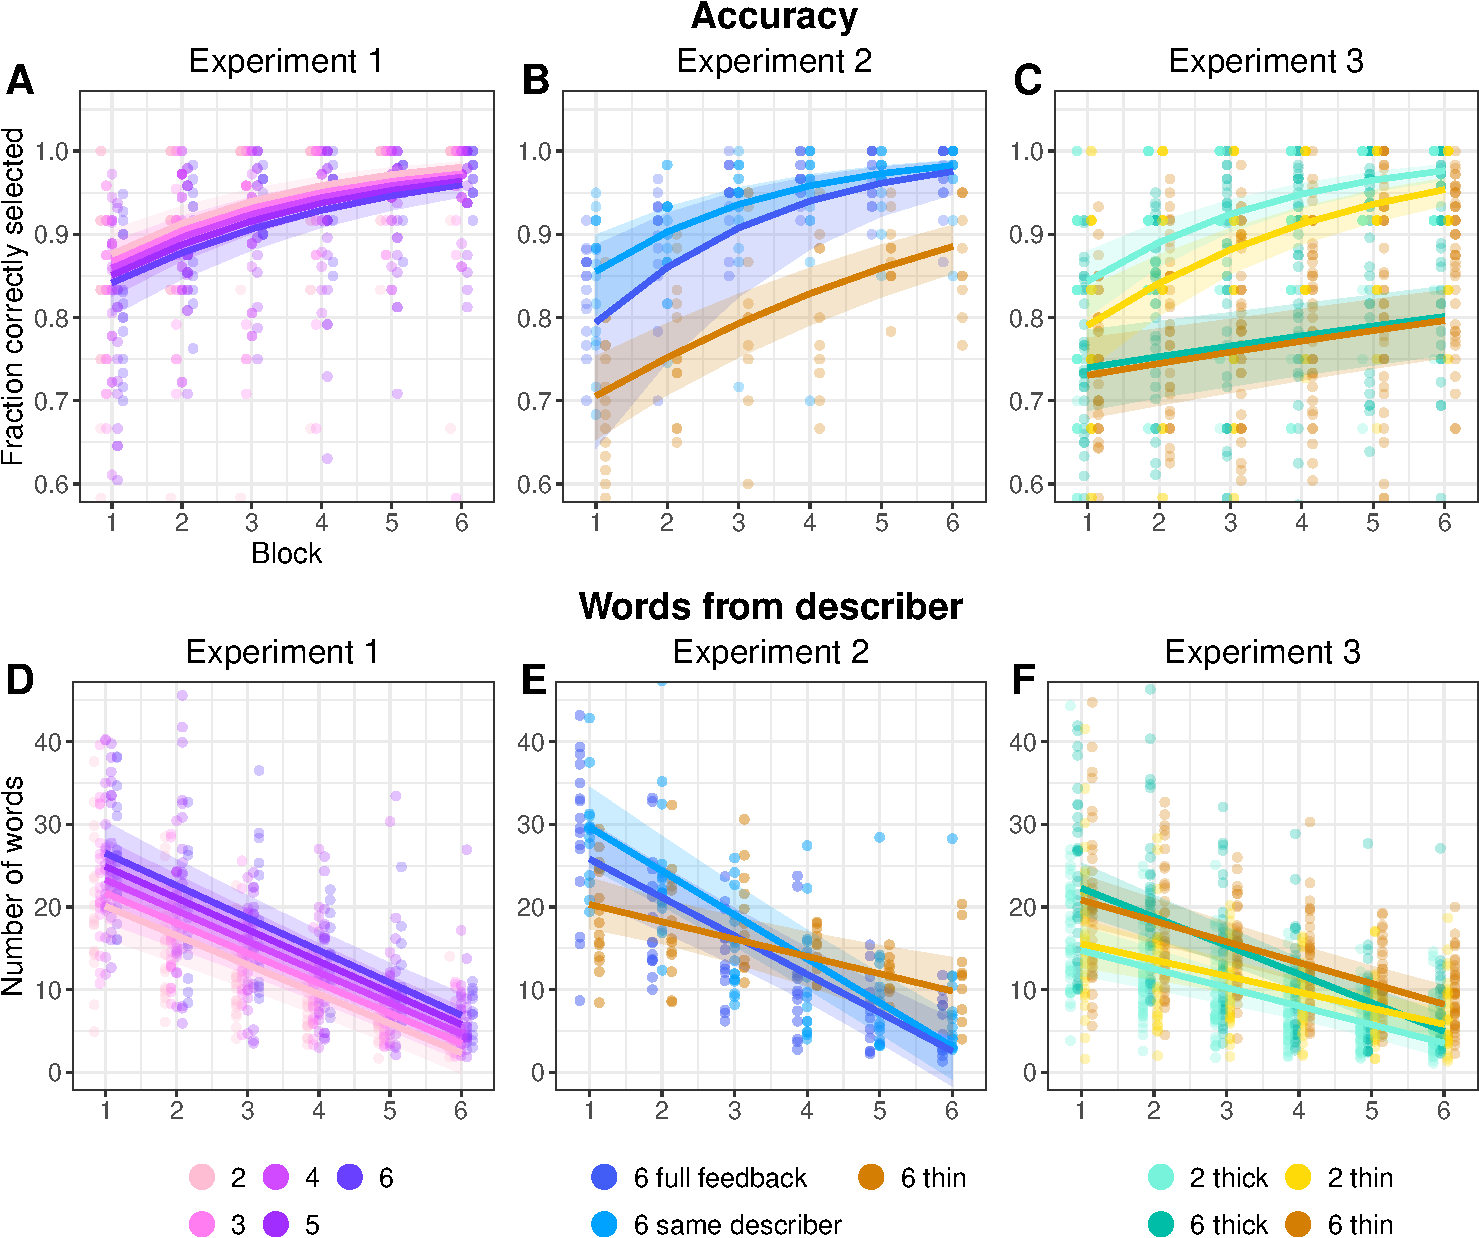
\includegraphics[width=.75\linewidth]{behavioral-1}\end{center}}

SI Figure 5:

          	{\begin{center} 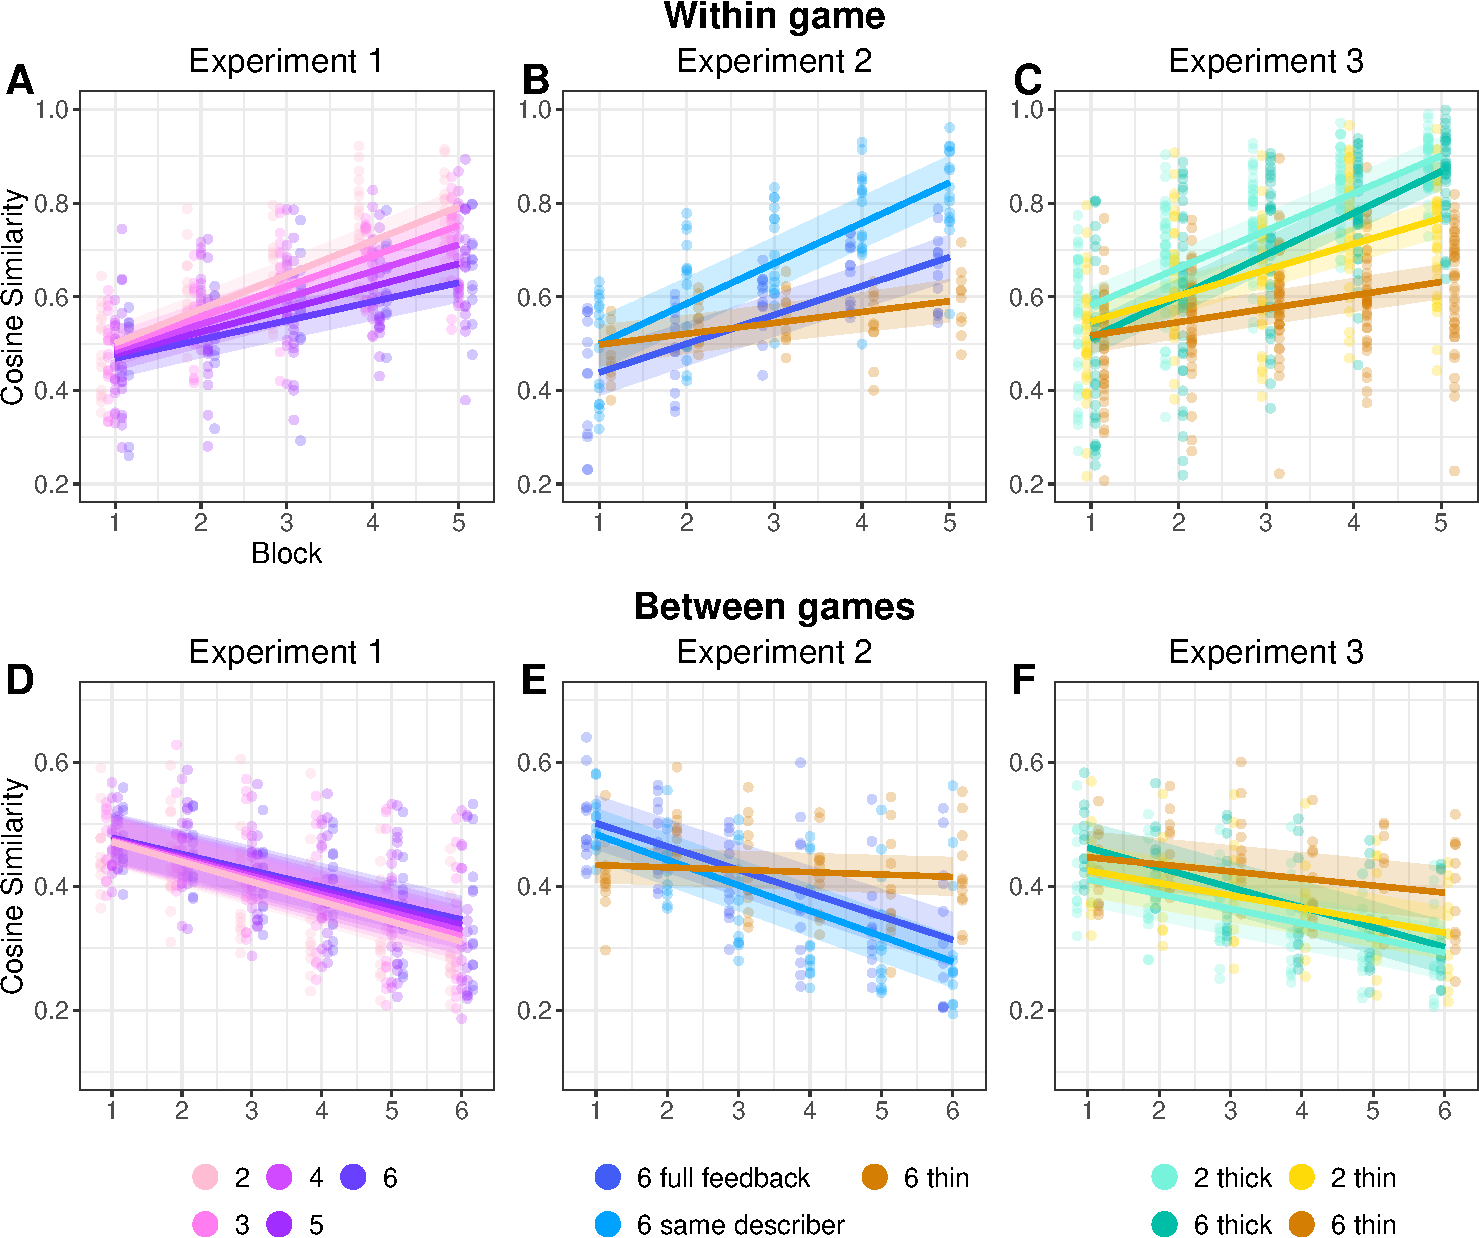
\includegraphics[width=.75\linewidth]{sbert-1}\end{center}}
          
          We added the following text to the Methods section explaining this additional analysis:
          

          \revised{As a sensitivity analysis, we re-ran the primary models on the subset of the data from games that a) completed all 72 trials and b) had the full complement of players the entire time (relevant to 6-player experiment 3 games where games could start or continue with fewer players). Discrepancies are mentioned in the results, and these analyses are depicted in SI Figures 4 and 5 and SI Tables 54-73.}
          
          For the most part, the model results were qualitatively the same and quantitatively similar to the results on the full sample. Where there were differences, such as when an effect reported in the main text had a Credible Interval overlapping 0 in the sensitivity analysis, we now mention in the main Results text that the certain result is not robust to the sensitivity analysis. 


          Addition to the ``Smaller and higher-coherence groups are more accurate'' section: 
          \revised{In Experiment 3, larger games began with
          	lower initial accuracy ($\beta$ = −0.64, 95\% CrI = [−1.05, −0.25]) and improved more slowly ($\beta$ =
          	−0.34, 95\% CrI = [−0.43, −0.25]) than smaller games, although group size differences were not
          	reliable in Experiment 1 (SI Table 4), and these experiment 3 differences were not robust in a 
          	sensitivity	analysis (SI	Figure 4C and SI Table 58).}
          
          
          Addition to the ``Smaller and higher-coherence groups are more efficient'' section: 
          \revised{In
          	Experiment 3, larger groups reduced faster than smaller ones ($\beta$ = −1.22, 95\% CrI = [−2.06, −0.29]),
          	but the faster reduction did not fully make up for the longer initial starting point, and was not robust to a sensitivity analysis (SI Figure 4F and SI Table
          	63).}
          	
          	Addition to the ``Descriptions converge faster in groups with thicker channels'' section: 
          	\revised{In Experiment 3, 6-person thick games started off further
          		from their eventual convention than 2-person thick games ($\beta$ = −0.069, 95\% CrI = [−0.113, −0.025])
          		but closed the gap over time (Figure 4C, $\beta$ = 0.009, 95\% CrI = [0.001, 0.017], this effect was not robust to sensitivity analysis,
          		SI Figure 5C and SI Table 68).}
          	
          \theysaid{- In the method, the time it took for each participant to click the target was recorded. Were they also analyzed? If so, is the result comparable to the result of describers' expression length (e.g., longer expressions lead to longer reaction time)? Or does the group size somehow modulate it?}
          
          
          We analyzed the reaction time data for at least experiment 1 as we were running experiments, but never specified it as a main analysis. 
          
          We have added a section to the Supplement with figures showing the RT for each matcher and the trial length of the whole group (equal to the slowest matcher). We also added a figure about the trial speed and number of words from the describer; these show a consistent relationship across conditions. 
          
          We added a brief mention of these results to the main text in the results section ``Smaller and higher-coherence groups are more efficient'':
          
          \revised{The reduction patterns of description lengths is paralleled by how long matchers took to make selections; across conditions, matchers selected faster in later conditions (SI Figure 9), and the correlation between speed and description length was consistent across experiments (SI Figure 10).}
          
          \theysaid{- Minor point: The resolution of Figure 1A is low, making it difficult to read text in the figure.}
          
          Thanks for bringing this up -- we have re-created Figure 1A and made it slighltly more schematic so that the text is a readable size. 
          
          \theysaid{Reviewer \#2:}
          \theysaid{Comments:}
          \theysaid{This is a very strong, well-written paper that explores a number of important issues relevant to reference and communicative dynamics. While there has been a wealth of research looking at communication processes in dyadic interactions, there has been relatively little psycholinguistic investigation into the nature of larger group interactions. The most substantial contributions of this work, therefore, lies in the way it systematically explores not only how group size affects the ability of interlocutors to efficiently develop communicative conventions, but also how such patterns of convergence are influenced by specific affordances of the communicative context. While I don't think anyone would find it surprising that 'thin' communication contexts result in less efficient interactions, it is nevertheless revealing to see how these constraints on communication interact with group size in interesting ways. This is a really nice set of results that expands our understanding of the dynamics of how interlocutors establish referential conventions. The contributions of this work are further strengthened by the methodological and analytic sophistication applied to the experiments, which are clever and appropriate for the questions being asked. I especially appreciated the use of sentence embeddings to derive a measure of semantic similarity for descriptions produced both within and between groups - this is an innovative way to show concretely not only how conventions emerge within groups but also how the nature of item descriptions begin to diverge across groups as they develop idiosyncratic ways of referring. All told, I like this paper, and only have a few, minor additional comments and suggestions.}
          
          
          \theysaid{p. 5, line 128ff: In the brief overview for Experiment 2, when I initially read "We manipulated two factors that we expected to increase group coherence...." I was imagining two clear independent manipulations within the same experiment - e.g., same describer vs. rotating describer or full feedback vs. impoverished feedback. This may be my fault, but it wasn't until the fuller description of this study on p. 14 that I came to understand that these manipulations were actually being implemented in comparison to what was done in Experiment 1. Similarly for line134: "We also manipulated a factor that...". I would suggest somehow making it clearer here that there were three conditions, each of which represented a critical change to one factor that was expected to impact group coherence.}

Thanks for letting us know that this paragraph was confusing. We have reworked the explanation of Experiment 2 to be more clear that there were 3 independent sub-experiments varying different factors. 

This part of the ``Overview of experiments'' subsection now reads: 
          
          \revised{Experiment 2 focused on the most challenging 6-player groups and explored the role of interaction structure. Each condition in Experiment 2 varied one aspect of the experiment relative to the Experiment 1 6-player baseline. We tried two variants that we expected to increase group coherence and improve performance, and a third variant we expected to interfere with the ability to establish mutual understanding and thus impede performance.
          	In the first variant, we maintained the same describer throughout rather than a rotating describer, such that the same individual has the opportunity to aggregate feedback across trials and track which matchers are struggling with which targets.
          	In the second variant, we gave the group of matchers full feedback about what every other member of the group had selected, and we showed the intended target.
          	In the third variant, we changed how matchers could make contributions to the group. In contrast to prior experiments, where matchers could contribute freely to the chat; here, we limited matchers to sending four discrete emojis (green check, thinking face, red x, and laughing-crying face) that could convey simple valence and level of comprehension, but not any referential content.}
          
          \theysaid{p. 7, concerning the conclusion that larger groups made greater use of backchannels - How can this be separated from the fact that larger groups also simply had more matchers available to backchannel?}
          
          
          This is a very good point. 
          We are more interested in the net volume of matcher contributions since this is what the describer experiences (how much response do they get from matchers?), so we focused on the group-level of how frequent and voluminous matcher contributions are. 
          
          However, the reviewer's question made us wonder what the analysis would look like on a per-matcher level. One could imagine that matchers might say less in larger groups (other matchers are on top of it already) or more (more content to chime in on, more options for matcher-matcher exchanges). 
          
          We added visualizations on the per-matcher level  (SI Figure 7) as well as running the same analyzes at the per-matcher level. Interesting, it turns out that an individual matcher in a large game is more likely to make a contribution than a matcher in a smaller game, suggesting that the number of matcher contributions scales super-linearly with the size of the game (SI Table 18). However, matchers in larger games say less per contribution than matchers in smaller games (SI Table 20). 
         
          We have revised the main text, which now reads:
          
          \revised{Overall, we found that larger groups displayed a higher proportion of trials where at least one matcher produced utterances (SI Figure 6A, \(\beta=0.79,\:95\%\:\mathrm{CrI}=[0.58, 0.98]\)), which declined across repetition blocks (\(\beta=-0.8,\:95\%\:\mathrm{CrI}=[-0.97, -0.62]\)). On an individual level, a matcher in a larger group was more likely to make contributions than a matcher in a smaller group, although each contribution tended to be shorter (SI Figure 7, SI Tables 18, 20).
          	The length of matcher interjections also decreased over time, especially for large groups (SI Figure 6D, \(\beta=-0.41,\:95\%\:\mathrm{CrI}=[-0.72, -0.11]\)) consistent with the need for early matcher involvement in establishing referential conventions.
          	Emoji use in Experiment 3 followed similar trends (SI Figure 8).
          	Overall, describers in larger groups receive more total input from matchers, suggesting larger groups may require greater participation by matchers to reliably establish common ground.}
         
          
          \theysaid{As mentioned above, I liked the analyses examining semantic similarity of describers' utterances within and between groups. I wondered, though, whether it would be possible to have more qualitative information about the nature of the actual descriptions, with an eye toward a more concrete understanding of how describers may have chosen to accommodate their utterances to the demands of the communicative situation. On p. 11, the paper alludes to the fact that initial similarity of descriptions across groups could have been higher because describers focused on 'shapes or body parts.' This reminded me of Fussell \& Krauss (1989), which found that speakers showed a relative preference for literal/geometric descriptions of novel images (vs figurative/holistic labels) when the descriptions were for an unfamiliar recipient, for whom a 'generic' description might be more appropriate. All else being equal, talking to a larger group or knowing that matchers may be restricted in what they can say may similarly prompt speakers to be more conservative in their descriptions, leading to an emphasis upon context-independent features that may be presumed to be equally available to addressees. Conventions can be based on different kinds of semantic perspectives. Basically, I would be interested in having a more fleshed out picture of the description content, if possible.}


          Thank you for this suggestion. The transcript text is quite long (more than 300 thousand words across all the games), so there's a limit to how deeply we can look at the content in the current paper. 
          
          We hope that the transcript is a resource for future work than can dive more in depth into what's going on with the convention formation than we are able to in a revision. 
          
          However, as a first step at getting a more concrete understanding of how the language is changing over time in different conditions, we did do a dictionary-based search for a few classes of words. These classes were chosen based on some pilot work trying to classify the types of descriptions in a portion of this dataset, and we think they reveal something about what types of description are being used. 
          
                    A new SI section contains a figure of the results and the following description of the methods:
          
          \revised{As an exploratory, qualitative analysis of the describer's language, we performed dictionary searches to classify whether the describers utterances on each trial contained the following types of words. 
          	
          	Geometric/literal words: squar*, triangle, triangular, diamond, shape, trapez*, angle, degree, parallel*, rhomb*, box, cube, line, white, black
          	
          	Words for body parts: face, head, heads, back, shoulder, shoulders, arm, arms, leg, legs, foot, feet, body, knee, knees, toe, toes, hand, hands, body, butt, heel, heels, ear, ears, nose, neck, chest, hair
          	
          	Positional words: right, left, above, below, under, over, top, bottom, behind, side, beneath
          	
          	Posture words: kick*, crouch*, squat*, kneel*, knelt, stood, stand*, sit*, sat, lying, walk*, facing, fall*, looking, lean*, seat*, laying
          	
          	Qualitatively, descriptions that contain none of these words are usually shorter, more abstract, more conventionalized descriptions. 
          	Figure 2 shows the fraction of trials where the speaker used these words. Generally, the more concrete word categories become less frequent over time, although this effect seems weaker in larger, thinner games. }
          	
          	SI Figure 2:
          	
          	{\begin{center} \includegraphics[width=.75\linewidth]{words-1}\end{center}}
          
          At the end of the main text Results section `` Games with thicker channels diverge from one another more quickly'', we have added:
          
          \revised{As a complement to the embedding analysis, we also examined the frequency of a few classes of words in the descriptions. Literal geometric words (ex. square, triangle, etc) and words for body parts (leg, arm, etc) are common early in games, but decline over repetition in most conditions, to be replaced by more abstract descriptions that do not contain these classes of words (SI Figure 2). The 6-person thin condition, however, retains a higher level of literal geometric and body part words, along with high levels of positional words (above, left, below, etc) and posture words (kicking, standing, seated, etc), with a lower level of utterances that do not contain any of these classes of words.
          }
          
          And in the discussion:
          \revised{The transcripts for these games provide a rich dataset for exploring different ways language is used to form referential conventions. }
          
 We hope our revisions to the text and addition the Supplementary Information have offered the necessary clarifications. We thanks the reviews and editors for their thoughtful feedback on this paper, which we deeply appreciate. 
          %TODO High resolution figure files are required for the final version of your manuscript. 
          
          %PNAS figure preparation guidelines state that no specific feature within an image may be enhanced, obscured, moved, removed, or introduced. The grouping or consolidation of images from multiple sources must be made explicit by the arrangement of the figure and in the figure legend. Adjustments of brightness, contrast, or color balance are acceptable if they are applied to the whole image and if they do not obscure, eliminate, or misrepresent any information present in the original, including backgrounds. Please note that our production editors may flag figures that are not in compliance with our figure policy, resulting in delays. For more information on submitting high resolution figures please review the PNAS digital art guidelines.
          



%TODO retag repo with new revision screenshot
          
          \closing{Sincerely,}
	\end{letter}
	
\end{document}




